
\chapter{Introduction}
\label{chapter_introduction}



%%%%%%%%%%%%%%%%%%%%%%%%%%%%%%%%%%%%%%%%%%%%%%%%%%%%%%%%%%%%

\section{Overview}


The continued increase of computing resources available for scientific and industrial research has motivated the simulation of complex flows. Several attempts have been done in order to fully simulate water-related hazards, from the its generation to its interaction with structures.

Usually, water-related hazards involve floods, which are complex natural phenomena with a great assortment of causes and a huge casuistic depending on the land characteristics or the climatic conditions. Preventing floods is still a great challenge due to uncertainty of climatic conditions and complexity of modeling land, usually defined by a great number of variables and parameters.

Furthermore, it is possible to identify several scales, local and global, whereas the local scale requires a high fidelity simulation. The identification of different levels of resolution makes the global simulation of these phenomena still unaffordable. From one side, the event generation can be global or local. If it is local, a \emph{Fluid-Structure Interaction} (FSI) simulation may be needed. The propagation of the event usually allows to assume several simplifications, corresponding to the large scale field. Finally, the interaction with structures is strictly a local scale.

\emph{Landslide-Generated Waves} (LGW) are an example of water-related natural hazards. Those events are originated when a landslide impacts a water reservoir and produces large-amplitude waves. LGW events can have devastating effects on the coastal areas of water basins, such as lakes, fjords and artificial reservoirs. Accurate modeling and prediction of LGWs are of key importance to reduce their catastrophic effects. Both experimental and numerical studies have been greatly contributed to the enhancement of the forecasting capabilities against these natural hazards. In that case, both the generation of the impulse wave and the interaction with structures require a local-scale resolution.

The direct simulation of all the scenario with a local scale resolution is computationally highly demanding and it can be unaffordable as long as the size of the scenario increases. This fact leads to the consideration of alternative strategies combining the numerical simulation of the large and local scale in a staggered frame. Figure \ref{space_time_staggered_approach} shows a conceptual identification of the different scales and the possible approaches. The computational cost is proportional to the area enclosed by the space-time domain and proportional to the efficiency of each solver. In Figure \ref{space_time_staggered_approach} the local-scale resolution is identified with a \emph{Near Field Solver} (NFS) and the large-scale resolution is identified with a \emph{Far Field Solver} (FFS).

The staggered approach, apart from being computationally more efficient, allows to decouple the uncertainty related to the generation from the FSI simulation. In addition, the staggered approach allows to concentrate the computational resources only where it is needed, thus having a more intelligent level of accuracy.


\begin{figure}
    \centering
    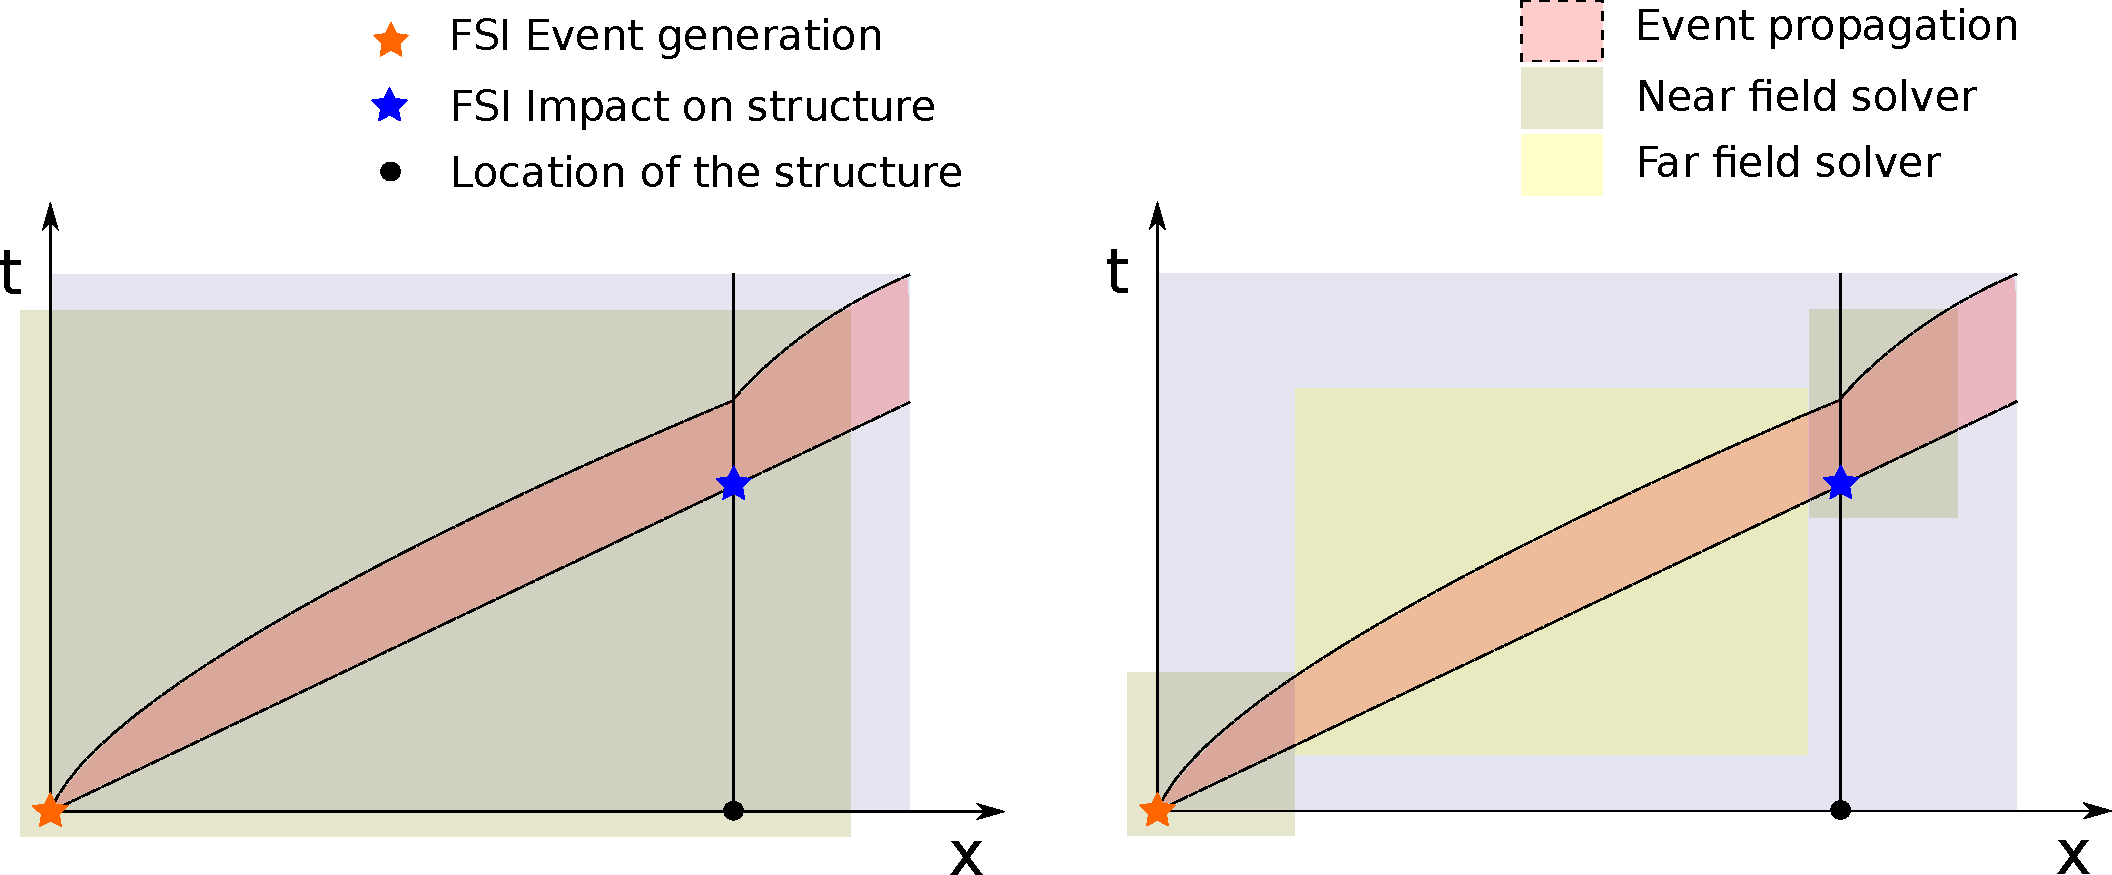
\includegraphics[width=\textwidth]{img/coupling/space_time}
    \caption{Propagation path of the event and possible computational approaches. Left: Brute force approach. Right: Staggered approach.}
    \label{space_time_staggered_approach}
\end{figure}


The main aspects that have been explored in this thesis are the numerical approximation of the FFS and the coupling strategy of the proposed FFS and an existing NFS. Special attention have been paid to the convergence and stability properties of the FFS aimed to solve the large scale.




%%%%%%%%%%%%%%%%%%%%%%%%%%%%%%%%%%%%%%%%%%%%%%%%%%%%%%%%%%%%

\section{Objectives and outline}


The work developed within the framework of this thesis can be enclosed in the global objective of investigating Finite Element formulations applied to large-scale water-related hazards. In particular, the analyzed methods have to be capable of reproducing local-scale effects around structures of interest and accurately model the large-scale propagation. This requirement lead to the analysis of the Finite Element Method for solving the Navier-Stokes equations on local scales and solving the shallow water equations on large scales.

The Navier-Stokes equations are typically solved using the finite element method, while the shallow water equations are often solved using the finite volume method.
Since we are interested in solving the global simulation within the same framework, a previous investigation on stabilized finite elements for the shallow water equations is presented.


This thesis is structured in 6 chapters, including the present introduction and a bibliographic revision. The bibliographic revision is specially extensive for the shallow water equations.
Chapter \ref{equations} presents a review of the governing equations which will be solved in the latter chapters.

Chapter \ref{eulerian_sw} is dedicated to the Finite Element Method applied to the shallow water equations. Stabilized formulations and quasi-monotonic formulations are presented.
Part of the developments of the numerical methods for the shallow water equations are moved to appendices \ref{lagrangian_sw} and \ref{mesh_refinement}, where the particle methods and mesh refinement are explored.
%This family of methods present some interesting properties, such as the natural approximation of the shoreline. The inconvenient of the Particle methods is the lack of robustness for all the possible flow regimes.

An extension of the shallow water equations to wave propagation on intermediate and deep water is presented in chapter \ref{eulerian_bsq}. These equations are known as the Boussinesq equations. The strategies developed in the previous chapter are applied to the Boussinesq equations, however, additional requirements must be fulfilled in order to ensure stability and accuracy. This chapter is of crucial importance in order to analyze impulse waves in the context of water-related hazards.

Chapter \ref{coupling} is devoted to the coupling strategies between the shallow water approximations --specially the Boussinesq equations-- and the fully resolved methods. An example of coupling for landslide long wave generation is provided.

Finally, the thesis is closed with some conclusions and possible further research lines in chapter \ref{conclusions}.


%%%%%%%%%%%%%%%%%%%%%%%%%%%%%%%%%%%%%%%%%%%%%%%%%%%%%%%%%%%%


\section{State of the art}
\label{state_art}


In this chapter a bibliographic revision of the methods employed to solve free surface flows problems is presented.
The analysis of the numerical methods for the shallow water equations is more extensive than the review for the Navier-Stokes equations, since this thesis presents some advances in the numerical simulation of the shallow water equations.



\subsection{Numerical methods for the Navier-Stokes model}

% \subsubsection{Overview}

% \subsubsection{Particle methods}



\subsection{Numerical methods for the shallow water models}


\subsubsection{Overview}

The computation of the dry-wet interface of the shallow water equations is a challenging problem. Due to the hyperbolic character of the equations the water height requires positivity ($h>0$) and oscillations can trigger global failure of the system. Löhner \cite{lohner2008} made a review of possible approximation methods to solve fluid dynamics. Being $u^h = N^i\hat{u}_i$ ($i=1,2,\dots,m$) an approximation of the solution $u$, the weighted residual is defined as

\begin{equation}
\int_{\Omega} W^ir(u^h)d\Omega = 0
\end{equation}

\begin{table}
\centering
\begin{tabular}{|l|c|c|}
\hline
 & $N^i$ & $W^i$ \\ \hline
Finite differences (FD)         & polynomial & $\delta(x_i)$ \\ \hline
Finite volumes (FV)             & polynomial & $1 \ \text{if} \ x\in\Omega_{el}$ \\ \hline
Galerkin finite elements (FEM)  & polynomial & $N^i$ \\ \hline
Discontinuous Galerkin (DG)     & polynomial & $N^i \ \text{if} \ x\in\Omega_{el}$ \\ \hline
\end{tabular}
\caption{Possible choices of trial and test functions $N^i$ and $W^i$}
\label{possible_trial_functions}
\end{table}

In table \ref{possible_trial_functions} there are a set of possible trial and test functions and the resulting approximation method. In the recent decades a new family of finite elements have been developed which are known as the discontinuous Galerkin (DG). We are interested on the implementation of \emph{continuous Galerkin finite elements} in KratosMultiphysics.


\subsubsection{Stabilized methods}



\subsubsection{Monotonicity preserving finite elements}

Following Löhner review, there are three classical approaches: stabilized finite elements \cite{lohner2008}, flux corrected transport (FCT) \cite{lohner2008ch9} and edge based finite elements \cite{lohner2008ch10}.

\paragraph*{Stabilized FEM} Streamline-diffusion methods like SUPG are stable but not
monotonicity preserving. However, Badia and Hierro presented a monotonicity preserving stabilized finite element for hyperbolic equations \cite{badia2014}.

\paragraph*{FCT} The way to circumvent the Godunov barrier theorem \cite{godunov1959} is to develop a nonlinear scheme. FCT uses a low order (LO) monotonic scheme with a lot of diffusion and a high order (HO) oscillatory scheme. The process of combining the two schemes is called limiting:

\begin{equation}
\phi^{n+1} = \phi^n + c_e\Delta \phi_H + (1-c_e)\Delta \phi_L
\end{equation}

\paragraph*{Edge based} The edge based structure is an efficient way to assemble the system matrix which resort to a
finite volume approximation of convective terms. If it is assumed that the fluxes of the variables are constant along the edges, a discontinuity will occur at the edge midpoint. Then, one can replace the Galerkin flux by a Riemann flux and obtain a total variational diminishing scheme (TVD).


% \subsubsection{Particle methods}



\subsection{Coupling strategies}




%%%%%%%%%%%%%%%%%%%%%%%%%%%%%%%%%%%%%%%%%%%%%%%%%%%%%%%%%%%%

\section{Research dissemination}


Some of the developments if this thesis have been published in the format of articles in peer reviewed journals. Since the research has advanced gradually, the articles are related to a chapter, but there are some differences, which can be big.
The chapters are more extensive than the articles and some parts of the articles are omitted to avoid repetitions.
There is also not the same sequence between the publication date and the chapter order.
On the other hand, since the notation is introduced gradually, it has been unified in the thesis and may be slightly different from the articles and this document.

\paragraph{Chapter \ref{eulerian_sw}} \fullcite{maso2022}
\paragraph{Chapter \ref{coupling}} \fullcite{maso2022b} (preprint)
\paragraph{Appendix \ref{lagrangian_sw}} \fullcite{puigferrat2021}
\\

In addition, the content of the chapters has been also disseminated in the form of oral presentations in scientific conferences and congresses:

\paragraph{Chapter \ref{coupling}} \fullcite{wccm2022}
\paragraph{Chapter \ref{coupling}} \fullcite{cmn2022}
\paragraph{Chapter \ref{coupling}} \fullcite{eccomas2022}
\paragraph{Appendix \ref{lagrangian_sw}} \fullcite{particles2019}

